\documentclass[a4paper]{article}

\usepackage[utf8]{inputenc}
\usepackage[portuguese]{babel}
\usepackage{graphicx}
\usepackage{amsmath}

\title{Projeto de Laboratórios de Informática 1\\Grupo 31}
\author{Henrique Manuel Palmeira Pereira (a80261) \and Ricardo Filipe Sousa Caçador (a81064)}
\date{MiEI - 1º Semestre}

\begin{document}

\maketitle

\tableofcontents

\section{Introdução}
No âmbito da unidade curricular Laboratórios de Informática I, foi-nos proposta a programação do jogo Bomberman (utilizando o Haskell) e a construção dos seus gráficos (recorrendo à biblioteca Gloss), de forma a ser possível jogar em Battle Mode, ou seja, entre um e quatro jogadores no mesmo teclado, com a possível existência de bots.

O trabalho foi dividido em seis partes pelos professores da UC, sobre as quais iremos falar no presente relatório. A primeira, descrita na secção \ref{t1}, foi onde programamos a construção dos mapas do jogo através da sua dimensão e de uma \textit{seed}. Na segunda, explicitada na secção \ref{t2}, definimos o movimento de um jogador. Na terceira parte, sobre a qual iremos falar na secção \ref{t3}, tivemos que programar o \textit{encode} (comprimir o estado de jogo, passando de uma lista de Strings para uma String apenas) e o \textit{decode} (partindo da String dada pela \textit{encode}, devolve novamente a lista de Strings original) do jogo. Na parte quatro do projeto (explicada na secção \ref{t4}), foi-nos pedido que programássemos a passagem do tempo no jogo. A quinta parte, que diz respeito à secção \ref{t5}, foi onde criamos os gráficos da nossa adaptação do jogo Bomberman, recorrendo a funções definidas nas restantes partes do trabalho. Na sexta e última parte, dada a conhecer na secção \ref{t6}, tivemos de programar um bot, de forma a que este "combata" com os bots dos restantes grupos e para que seja possível jogarmos sozinhos o jogo em questão.

Para facilitar a programação das Tarefas 4, 5 e 6, foram criados três módulos com as funções definidas por nós nas tarefas anteriores. Os módulos encontram-se na pasta /src, junto dos ficheiros .hs do projeto.

As principais funções de cada parte estão explícitas na seguinte tabela:

\begin{table}[h]
	\centering
\begin{tabular}{|r|l|}
	\hline
	\textbf{Nome} & \textbf{Descrição} \\ \hline
	\texttt{mapa} & função da tarefa 1 \\ \hline
	\texttt{move} & função da tarefa 2 \\ \hline
	\texttt{encode e decode} & função da tarefa 3 \\ \hline
	\texttt{avanca} & função da tarefa 4 \\ \hline
	\texttt{bot} & função da tarefa 6 \\ \hline
\end{tabular}
\caption{Funções}
\end{table}
\label{tb1}

\section{Tarefa 1}
\label{t1}
A Tarefa 1, como foi dito na introdução, corresponde à construção de um mapa de Bomberman, mapa este que consiste numa lista de Strings, dispostas por ordem de linhas do mapa. 

Assim sendo, no mapa estão presentes quatro caracteres: 
\begin{itemize}
\item ‘\#’ - corresponde às pedras fixas do mapa, que não são possíveis de rebentar com bombas e que se encontram sempre na mesma posição qualquer que seja a semente geradora do mapa;
 \item '?' - corresponde aos tijolos (ou caixas) que podem ser explodidas e que podem esconder power-ups, variando consoante a semente dada;
 \item '+' - corresponde aos power-ups Bombs;
 \item '!' - corresponde aos power-ups Flames.
\end{itemize}

\subsection{Função mapa}
A principal função desta tarefa é a \texttt{mapa} que recebe como inputs a dimensão do mapa e uma semente e devolve um mapa (lista de Strings).
Recorrendo a funções auxiliares das bibliotecas System.Environment, Text.Read, Data.Maybe, Data.List, System.Random, Data.Char e a outras por nós definidas. 

Começamos por definir o mapa gerando os valores fixos, isto é, dispondo as pedras nos seus lugares. Após isso, introduzimos os valores gerados pela semente, tais como as caixas e os power-ups.

Desta maneira, definimos a função mapa da seguinte forma:
\begin{verbatim}
mapa :: Int -> Int -> [String]
mapa d s = substituiMapa (mapa1 d s)++darCoordMapa1 d s 0++darCoordMapa2 d s 0
\end{verbatim}

\section{Tarefa 2}
\label{t2}
Na Tarefa 2, o objetivo era programarmos a função \texttt{move}, que consiste em fazer com que os jogadores se desloquem ou coloquem bombas no mapa. Segundo o enunciado, os caracteres que permitiam o movimento dos jogadores é o seguinte:
\begin{itemize}
\item 'U' - movimenta o jogador para cima
\item 'D' - movimenta o jogador para baixo
\item 'L' - movimenta o jogador para a esquerda
\item 'R' - movimenta o jogador para a direita
\item 'B' - coloca uma bomba na posição do jogador.
\end{itemize}

\subsection{Função move}

Para obtermos o pretendido, tivemos primeiramente de arranjar maneira de retirar as coordenadas dos jogadores, das bombas, das pedras, das caixas e dos power-ups do mapa, para vermos se é possível ou não o movimento, isto é, se, por exemplo, um jogador tiver um tijolo em cima dele e quiser andar para cima, não o pode fazer. Após verificarmos a possibilidade de movimento, tivemos que programar a colocação de bombas no mapa, sendo que cada jogador pode apenas pôr uma bomba de cada vez (se não tiver apanhado nenhum power-ups Bombs) e que não é possível colocar uma bomba em cima de outra. Além disso, tivemos também de fazer com que o jogador apanhasse power-ups quando passa por cima deles, eliminando assim as suas informações do estado de jogo.

Contudo, só após o término da data de entrega da primeira fase do projeto é que descobrimos um erro no nosso código, que não permitia alguns movimentos nos mapas de dimensão superior a 9. Esse erro foi de imediato corrigido, não apresentando agora a função \texttt{move} qualquer problema de funcionamento.

Desta maneira, definimos a \texttt{move} da seguinte forma:
\begin{verbatim}
move :: [String] -> Int -> Char -> [String]
move [] j m = []
move mapa j m  | m == 'B'  && (ifFlames mapa j == True) 
        && bombasJogadorMapa mapa j <= contarB (tirarCoord mapa j)   
        = ((cardinais mapa) ++ (listapowerups mapa) 
        ++ (insert (tuploDeixarBombaF j (tuplo (getCoord ( tirarCoord mapa j))) 
        (contarF (tirarCoord mapa j))) (bombas mapa)) 
        ++ listajogadores mapa)
               | m == 'B' && (bombasJogadorMapa mapa j) <= contarB (tirarCoord mapa j) 
        = (if elem (tuplo (getCoord ( tirarCoord mapa j))) (bIniciais mapa) == False  
           then ((cardinais mapa) ++ (listapowerups mapa) 
        ++ (insert (tuploDeixarBomba j (tuplo (getCoord ( tirarCoord mapa j)))) 
        (bombas mapa)) ++ listajogadores mapa)
           else  mapa)
               | m == 'B' && (bombasJogadorMapa mapa j) > contarB (tirarCoord mapa j) 
        = mapa
               | verificaJogador j (listajogadores mapa) == False = mapa  
               | elem (andar mapa j m) (tP mapa)== True = mapa 
               | elem (andar mapa j m) (coordB mapa) == True  
        = delete (tuploStringB (andar mapa j m)) (insert (tuploString j (andar mapa j m) 
        ++ " " ++ replicate (cMais (tirarCoord mapa j)) '+' ++ "+ "  
        ++ replicate (cFlames (tirarCoord mapa j)) '!'    )  
        (delete (tirarCoord mapa j) mapa)) 
               | elem (andar mapa j m) (coordF mapa) == True  
        = delete (tuploStringF (andar mapa j m)) (insert (tuploString j (andar mapa j m) 
        ++ " " ++ replicate (cFlames (tirarCoord mapa j)) '!' ++"! " 
        ++ replicate (cMais (tirarCoord mapa j)) '+' )  (delete (tirarCoord mapa j) 
        mapa)) 
               | elem (andar mapa j m) (tP mapa)== False 
        =  delete (tuploStringF (andar mapa j m)) (insert (tuploString j (andar mapa j m) 
        ++ " " ++ replicate (cMais (tirarCoord mapa j)) '+' 
        ++ replicate (cFlames (tirarCoord mapa j)) '!' ) (delete (tirarCoord mapa j) 
        mapa))       
               | otherwise = mapa
\end{verbatim}

\section{Tarefa 3}
\label{t3}

Na Tarefa 3, tínhamos que fazer com que o jogo pudesse ser pausado, "pesando menos" no computador, ou seja, tivemos de programar o \texttt{encode} do mapa, fazendo com que a lista de Strings, que é o estado de jogo, passasse a ser uma só String, com as informações essenciais lá guardadas.

Após isso, era necessário pegar nessa String e transformá-la de novo numa lista de Strings, fazendo com que o jogo voltasse ao estado em que estava no momento que foi pausado, isto é, tivemos que programar o \texttt{decode}.

\subsection{Funções encode e decode}
Ora, para obtermos o resultado pretendido, decidimos que podíamos descartar as informações fixas, umas vez que as pedras são facilmente obtidas a partir da dimensão do mapa e da semente, que guardamos na String. De seguida, decidimos que teríamos de guardar as informações relativas às posicoes das caixas, e, para isso, colocamos na String gerada pela \texttt{encode} as suas coordenadas. Além disso, para diminuirmos ainda mais o tamanho do estado de jogo, retiramos os espaços entre as informações dos power-ups, das bombas e dos jogadores.

Com tudo isto, a compressão por nós conseguida não foi a melhor, mas conseguimos reduzir o tamanho original em cerca de 35\%.

Definimos, portanto, a \texttt{encode} da seguinte maneira:
\begin{verbatim}
encode :: [String] -> String
encode l = unlines (mapaDim l ++ tirarEspaco (tirarConsec 
           (tEpVALL (separarCoordPU l))) ++ separarJog l)
\end{verbatim}

No que diz respeito à descompressão do estado de jogo, começamos por gerar novamente o mapa a partir da sua dimensão e da sua semente e de, seguida, colocamos as caixas nos devidos lugares, usando as coordenadas guardadas na String. Após esse processo, colocamos novamente os espaços nas informações adicionais do jogo.

Desta forma, a \texttt{decode} foi assim definida:
\begin{verbatim}
decode :: String -> [String]
decode l = substituiPontos (drop (length (ficaDim l)+1) l) 
       (mapaSemN 0 (read (ficaDim l))) 
           ++ lines ( tVpE (porSimbolo (ficarBombs (ficarInf (tirarJog l))) '+') 
           ++ tVpE (porSimbolo (ficarFlames (resto (ficarInf (tirarJog l)))) '!')
           ++ tVpE (porSimbolo (ficarBombas (resto (ficarInf (tirarJog l)))) '*')
           ++ ficarJog l )
\end{verbatim}

\section{Tarefa 4}
\label{t4}
O objetivo da Tarefa 4 era programar o efeito da passagem do tempo no jogo, ou seja, o efeito da explosão das bombas no mapa e a queda de pedras no mapa numa trajetória espiral, de forma a ir fechando o mapa à medida que o tempo do jogo se aproxima do fim. 

Segundo o enunciado, sempre que uma bomba explodisse e se encontrasse uma bomba dentro do raio da primeira, a segunda explodiria logo no instante seguinte, criando como que um efeito de dominó. Além disso, todos as caixas, jogadores e power-ups que se encontrem no raio de explosão de uma bomba são eliminados no momento de explosão da mesma.

Relativamente ao efeito de espiral, no momento em que faltam \((n-2)^2\), num mapa de dimensão \(n\), começam a cair pedras no mapa, fazendo uma espiral, de maneira a fechar o mapa para forçar os jogadores a acabar o jogo.

\subsection{Função avanca}
Desta maneira, começamos por retirar do estado de jogo as informações relativas ao tempo das bombas e, de seguida, aos raios. Depois, tivemos que retirar as coordenadas do que pode ser destruído, ou seja, jogadores, caixas e power-ups. Para os explodir, foi necessário comparar a posição da bomba e o seu raio com a posição das três coisas referidas anteriormente. Além disso, foi necessário fazer com que a explosão não atravessasse pedras, nem caixas, nem power-ups, sendo que a única coisa que pode desruir em simultâneo na mesma direção são os jogadores. Assim, uma bomba com mais que um de raio, não pode destruir duas caixas seguidas que se encontram lado a lado, na mesma linha, ou uma em cima da outra, na mesma coluna. Foi preciso também programar o "efeito dominó" das bombas que foi anteriormente explicitado, comparando o tempos das bombas dentro do raio daquela com menor tempo restante para a sua explosão.

Relativamente à espiral, começamos por desenvolver uma função que para cada inteiro (instantes que faltam para terminar o jogo) correspondesse uma coordenada, o que nos permitiu obter a primeira volta da espiral com facilidade. Após isso, desenvolvemos várias funções auxiliares para, partindo da primeira volta, completarmos as seguintes.

Definimos a função \texttt{avanca} da seguinte maneira:
\begin{verbatim}
avanca :: Mapa -> Int -> Mapa
avanca mapa x | x > ((length (head mapa)-2)^2) = if verBomba mapa == True 
    then cardinais (arrebentaPI mapa (explodePI (tI mapa) (tB mapa) mapa)) 
    ++ listapowerups (arrebentaPU mapa) ++ instanteBomba mapa ++ listajogadores2 
    (arrebentaBonecos mapa (explodeJ (tJ mapa) (tB mapa) mapa))
    else  cardinais mapa ++ listapowerups mapa ++ instanteBomba mapa 
    ++ listajogadores2 mapa
              | x <= ((length (head mapa)-2)^2) && x>=1 = if verBomba mapa == True
    then cardinais (metePontoEspiral (arrebentaPI mapa (explodePI (tI mapa) 
    (tB mapa) mapa)) (espiral (length (head mapa))x))  ++ listapowerups ((removeGeral 
    (espiral (length (head mapa))x)) (arrebentaPU mapa)) ++ instanteBomba (removeGeral 
    (espiral (length (head mapa))x) mapa) ++ listajogadores2 ((removeGeral  (espiral 
    (length (head mapa))x)) (arrebentaBonecos mapa (explodeJ (tJ mapa) (tB mapa) mapa)))
    else  cardinais (metePontoEspiral mapa (espiral (length (head mapa))x)) 
    ++ listapowerups ((removeGeral  (espiral (length (head mapa))x)) mapa) 
    ++ instanteBomba (removeGeral (espiral (length (head mapa))x)mapa) 
    ++ listajogadores2 ((removeGeral  (espiral (length (head mapa))x)) mapa)
              | otherwise = mapa
\end{verbatim}

\section{Tarefa 5}
\label{t5}
Na Tarefa 5 foi-nos proposta a criação de gráficos de modo a tornar o jogo executável, sendo esta a fase mais criativa do projeto. Para esse propósito, foi utilizada a biblioteca Gloss e algumas imagens em formato bitmap (\texttt{.bmp}), umas criadas por nós e outras retiradas da internet. A função principal utilizada foi a \texttt{play}, que pertence à biblioteca antes referida e é do seguinte tipo:
\begin{verbatim}
play :: Display
-> Color 
-> Int 
-> Estado 
-> (Estado -> Picture) 
-> (Event -> Estado -> Estado) 
-> (Float -> Estado -> Estado) 
-> IO ()
\end{verbatim}

Assim, começamos por definir um novo tipo de dados, que denominamos de \texttt{Estado}, onde colocamos toda a informação que nos seria útil para a criação do jogo. De seguida, definimos uma função do tipo Display que determinasse o tamanho da janela de jogo e a sua posição no ecrã. Após isso, decidimos a cor do fundo ("aquamarine") e o número de frame rates que achamos mais pertinente para o nosso jogo (que foi 5). O passo seguinte foi determinar o estado inicial do jogo, que é a primeira página do menu, ou seja, é o primeiro ecrã que nos aparece quando executamos o jogo. Após isso, definimos a função \texttt {desenha}, que, recebendo um \texttt{Estado}, vai transformá-lo numa imagem, a função \texttt{continua}, que permite a seleção de opções e o movimentação dos bonecos através do teclado do computador e a função \texttt{reageTempo}, que faz com que o tempo passe no jogo, atendendo ao frame rate por nós definido. Foi nesta última função também que nos foi possível também introduzir o bot por nós programado (sobre o qual iremos falar na secção \ref{t6}).

Para transformar o estado de jogo (\texttt{[String]}) numa imagem, começamos por desenhar o mapa, consoante a sua dimensão, desenhando no ecrã as pedras e as caixas. De seguida, colocamos os power-ups, ficando estes debaixo das caixas, e os jogadores no mapa, consoante as coordenadas referidas no estado de jogo, sendo os seus movimentos regulados pela função \texttt{move}. Depois, introduzimos as bombas no mapa e as respetivas explosões, tendo em conta o seu raio de explosão, o seu "cronómetro" e a função \texttt{avanca}. Para melhorar a jogabilidade do nosso Bomberman e o seu aspeto visual, acrescentamos um painel lateral ao jogo, onde consta o tempo que falta para terminar o jogo e os jogadores e respetivas informações (se se encontram vivos ou mortos, quantos power-ups têm e se são bots ou não).

Os controlos por nós definidos para jogar são os seguintes:
\begin{itemize}
\item Jogador 1
	\begin{itemize}
	\item Cima - W
	\item Esquerda - A
	\item Baixo - S
	\item Direita - D
	\item Bomba - Q
	\end{itemize}
\item Jogador 2
	\begin{itemize}
	\item Cima - KeyUp
	\item Esquerda - KeyLeft
	\item Baixo - KeyDown
	\item Direita - KeyRight
	\item Bomba - KeyEnter
	\end{itemize}
\item Jogador 3
	\begin{itemize}
	\item Cima - T
	\item Esquerda - F
	\item Baixo - G
	\item Direita - H
	\item Bomba - Y
	\end{itemize}
\item Jogador 4
	\begin{itemize}
	\item Cima - I
	\item Esquerda - J
	\item Baixo - K
	\item Direita - L
	\item Bomba - O
	\end{itemize}
\end{itemize}

Além disso, definimos um menu onde o utilizador pode selecionar o número de jogadores (1-4) e a dificuldade, que representa a dimensão do mapa, ou seja,
no modo principiante é um mapa de dimensão 7, no intermédio é de dimensão 13 e no profissional é de dimensão 17. A semente dos mapas é gerada aleatoriamente.

\section{Tarefa 6}
\label{t6}
Nesta última tarefa, foi-nos proposta a programação de um bot, que combatesse de maneira inteligente. A estratégia que decidimos implementar foi a seguinte: o bot desloca-se até ao centro do mapa (destruindo as caixas que se encontram no seu caminho), de forma a combater o efeito da espiral. Após a sua chegada, o bot fica à espera que cheguem os restantes bots, iniciando de seguida o modo ataque, colocando bombas no raio do jogador, esquivando-se das mesmas e das dos adversários.
\subsection{Função bot}
Ora, para obtermos esse resultado, tivemos que fazer o seguinte:
\begin{enumerate}
\item Fazer com que o bot se mexa;
\item Verificar o raio das bombas e afastar-se delas, deslocando-se para fora do seu raio;
\item Divisão do mapa em quatro quadrantes, de forma a controlar o bot dependendo da sua posição no mapa, ou seja, do quadrante em que se encontra;
\item Programar o bot para por bombas, explodir caixas e tentar matar os adversários.
\end{enumerate}

\section{Conclusão}

Em suma, este trabalho foi extremamente interessante, enriquecedor e entusiasmante para ambos os elementos do grupo, uma vez que nos estimulou a sermos autónomos e a programarmos um jogo, algo que a maior parte das pessoas gosta, e fez-nos ver o que está por detrás dos grandes jogos existentes no mercado e a complexidade da programação de um simples Bomberman em 2D. Além disso, foi uma excelente maneira de consolidarmos os nossos conhecimentos de Haskell e também de nos proporcionar a aquisição de novos.

O resultado final do jogo pode ser visualizado nas imagens seguintes.

\begin{figure}[h]
  \begin{center}
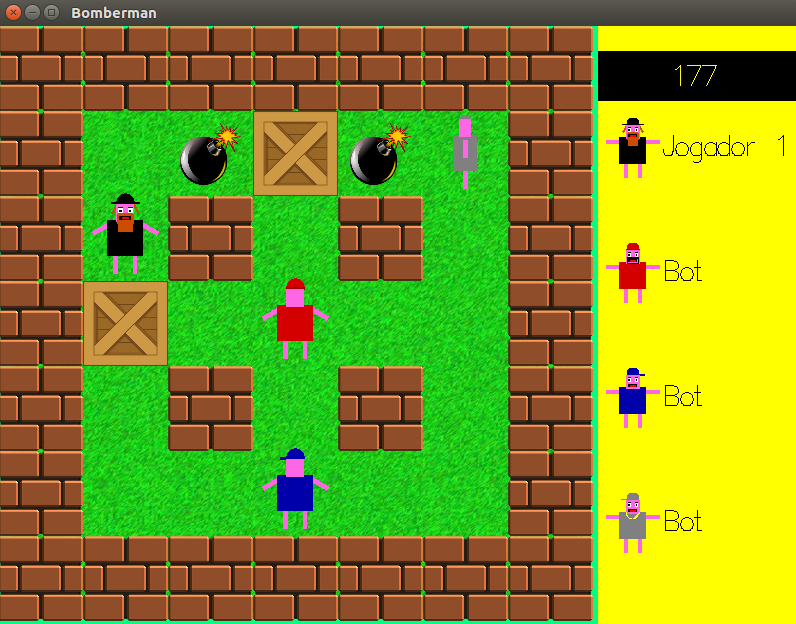
\includegraphics[scale=0.13]{imagem1.png}
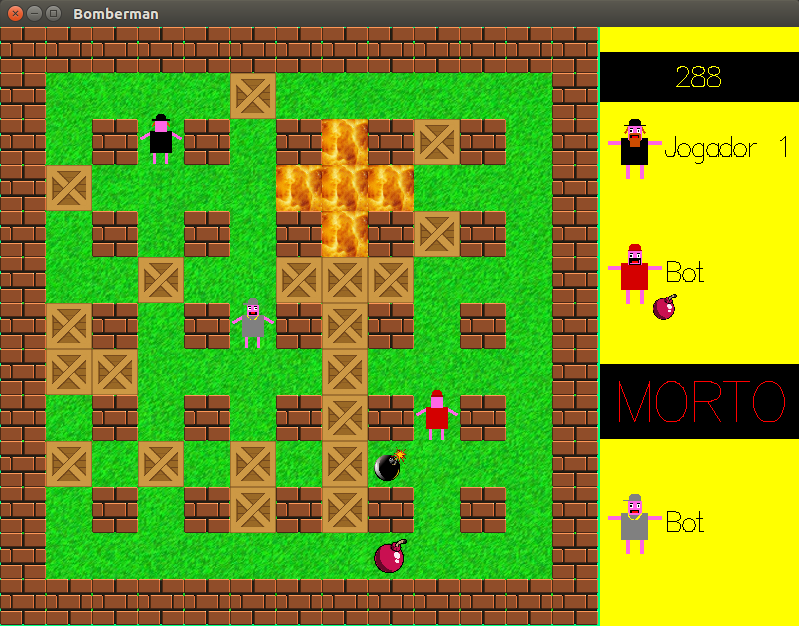
\includegraphics[scale=0.13]{imagem2.png}
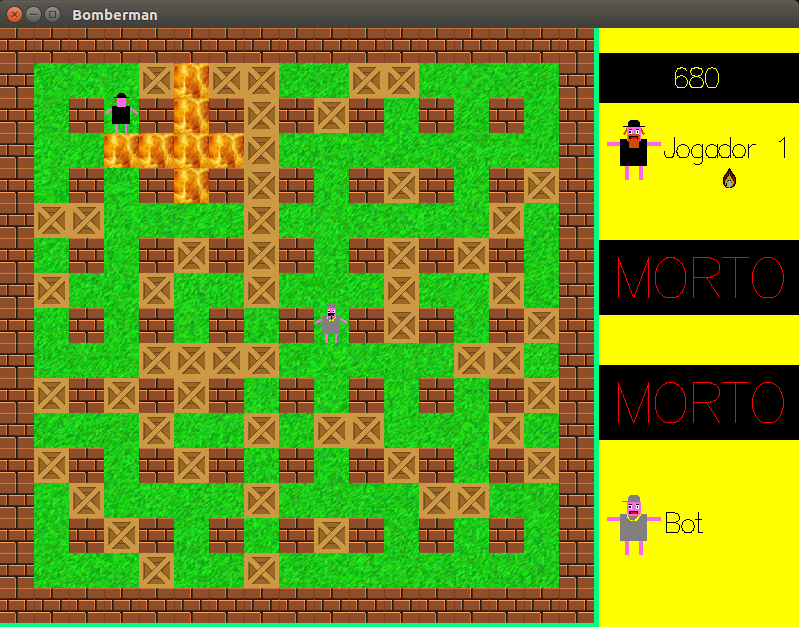
\includegraphics[scale=0.13]{imagem3.png}
\caption{Screenshots do jogo}
  \end{center}
\end{figure}

\end{document}\grid